\section{Baseline Details}
The details of our baselines are listed as follows:
\begin{itemize}
    \item D$^3$L \cite{bogatu2020dataset}  addresses the problem of finding related tables in data lakes by constructing a comprehensive similarity framework that utilizes multi-dimensional attributes such as column names, value overlap, and formatting features.  
    \item Sherlock \cite{hulsebos2019sherlock}  is a feature-based representation learning method that aggregates various micro-features, such as character embeddings, character distributions, and global table statistics, to map data columns into compact embedding vectors for semantic type detection. 
    \item SATO \cite{zhang2019sato} extends Sherlock by integrating an LDA topic model to explicitly capture global table context information, thereby performing multi-column prediction to significantly improve the robustness of semantic type detection. 
    \item SANTOS \cite{khatiwada2023santos} introduces a relationship-based approach for semantic table union search that goes beyond content matching by leveraging external and self-curated knowledge bases to infer deep semantic associations between columns.  
    \item TAPAS \cite{herzig2020tapas} extends the BERT architecture for tabular data by incorporating row and column position embeddings and utilizing a masked language modeling objective on flattened tables to achieve weakly supervised table parsing.  
    \item Doduo \cite{jiang2024doduo} builds upon a Transformer-based serialized table representation, employing a multi-task learning objective to simultaneously predict column types and column relations, thus facilitating knowledge sharing and complementarity between different semantic tasks.  
    \item Starmie \cite{fan2022semantics} presents a contrastive learning framework to generate contextualized column embeddings, utilizing serialized table content and a multi-column attention mechanism to effectively capture inter-column dependencies for optimizing table union search. 
    \item LIFTus \cite{qiu2025liftus} proposes an adaptive multi-aspect representation learning architecture that fuses linguistic features from pre-trained language models (PLMs), character-level patterns, and numerical distributions via a hierarchical cross-attention mechanism to handle heterogeneous data. 

    \iffalse
    \item w/o variance is our baseline encoder that only uses a deterministic point vector as the output of the encoder in the training process. This is DGGC (Full) without the distributional uncertainty modeling. 
    \item w/o wass is our distributional variant that utilizes the Gaussian embedding but ignores the geometric penalty in the training process. This is DGGC (Full) without the Wasserstein distance regularization. 
    \item w/o real pos is our unsupervised baseline that only uses single-table augmentation views as positive pairs in the training process. This is w/o variance without the relation-guided positive sampling. 



    \item DGGC (only header pos) is our modality variant that only uses schema information as the input of the encoder in the training process. This is DGGC (Full) without the data content information. 
    \item DGGC (only data pos) is our modality variant that only uses cell values as the input of the encoder in the training process. This is DGGC (Full) without the schema context information. 
    \item DGGC (Full) is our complete framework that utilizes both relation-guided sampling and Wasserstein distribution constraints in the training process. This is the optimal configuration incorporating all proposed components. 
    \fi

\end{itemize}

\iffalse
\end{itemize}
\section{Case Study}
\label{app:case_study}
\begin{figure}
    \centering
  
    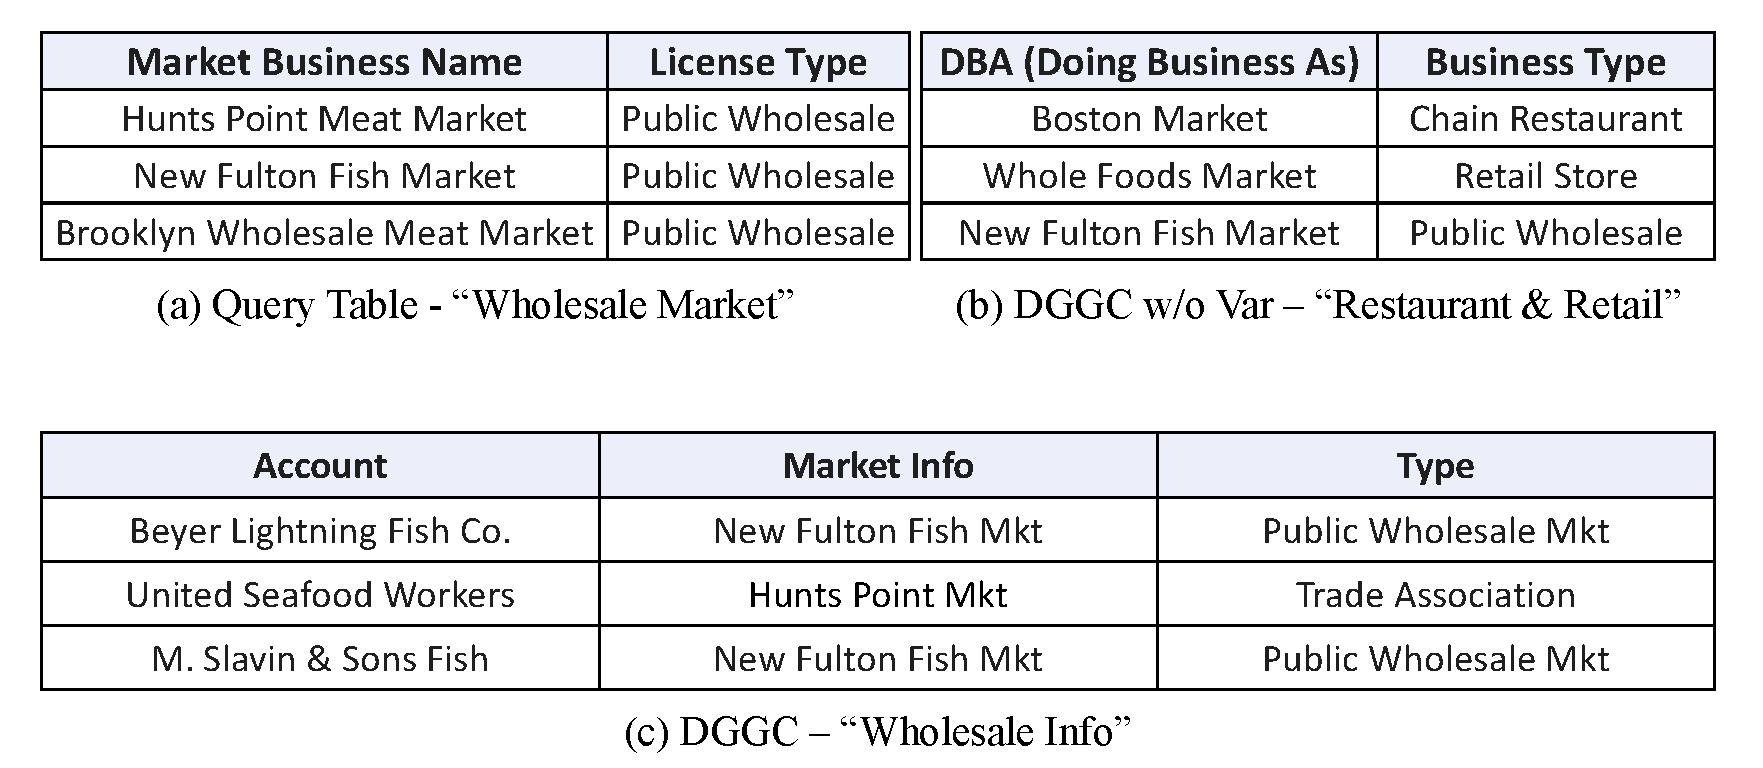
\includegraphics[width=1\linewidth]{figure/case_study.pdf}
    \caption{A case study of table union search: (a) The query table about ``Wholesale Markets''; (b) The returned table of DGGC w/o Var, which is a restaurant \& retail table due to its high lexical overlap with the query table (e.g., ``Market'', ``Type''); (c) The returned table of DGGC, which is a true positive containing markets with public whole sale type. }
    \label{fig:casestudy}
   
\end{figure}

To intuitively understand the superiority of our approach, we present a case study in Figure \ref{fig:casestudy} DGGC with the DGGC w/o Var. We analyze a representative query from the ``Wholesale Markets'' domain where lexical overlap introduces ambiguity.

As shown, the DGGC w/o Var model retrieves a ``Restaurant Inspection'' table as the top result. This occurs because the baseline relies heavily on keyword matching, thereby failing to capture the semantic boundary despite the severe lexical overlap (e.g., tokens like ``Market'' and ``Seafood''). Specifically, the point-based embedding projects these structurally different tables into close proximity due to shared high-frequency terms.



However, using the Wasserstein constraint (DGGC) successfully retrieves the correct target (\texttt{Wholesale Info.csv}). This suggests that our model effectively models the semantic variance of the schema. Specificall  y, the column \texttt{Account Name} in the query forms a distinct Gaussian distribution with low variance. While the baseline conflates this with the \texttt{DBA Name} in the restaurant table, the Wasserstein metric penalizes the alignment between these mismatched distributions. Thus, the transport cost \cite{peyre2019computational} required to align these distributions remains high, allowing the model to filter out the hard negative. This qualitatively confirms that modeling tables as probability distributions compensates for the limitations of simple semantic matching in high-ambiguity scenarios.



To intuitively understand the superiority of DGGC in handling semantic specificity in tables, we provide a case study focus on the tables about ``Wholesale Markets'', a domain where heavy lexical overlap frequently impacts the performance of union search. Figure \ref{fig:casestudy} presents the query table and the union search results by DGGC and DGGC w/o Var. Figure \ref{fig:case_study_epoch} shows the MAP of all queries, the cosine similarity between the mean embedding of the query table in the case study and its negative sample embedding as the epoch increases.

As illustrated in Figure \ref{fig:casestudy} and Figure \ref{fig:case_study_epoch}, the DGGC w/o Var retrieves a ``Restaurant \& Retail'' table, which is misled by severe value-level lexical overlap (estimated Jaccard similarity $\approx 0.42$). The overlapping strings, such as ``Hunts Point Meat Market'' vs ``Boston Market'', ``License Type'' vs ``Business Type'' create a high similarity between two tables. At Epoch 1, the cosine similarity between negative samples is notably high at 0.982. However, as training progresses, this similarity significantly drops to 0.2138 by Epoch 30. The overall MAP@k reaches its peak at Epoch 2 but subsequently begins to decline. This deterioration can be attributed to the model's neglect of semantic specificity due to the absence of a variance constraint. As a result, the model overfits to noise, leading to a gradual decrease in MAP@k performance, which falls from 0.9346 to 0.7054.

\begin{figure}[!htpb]
    \centering
    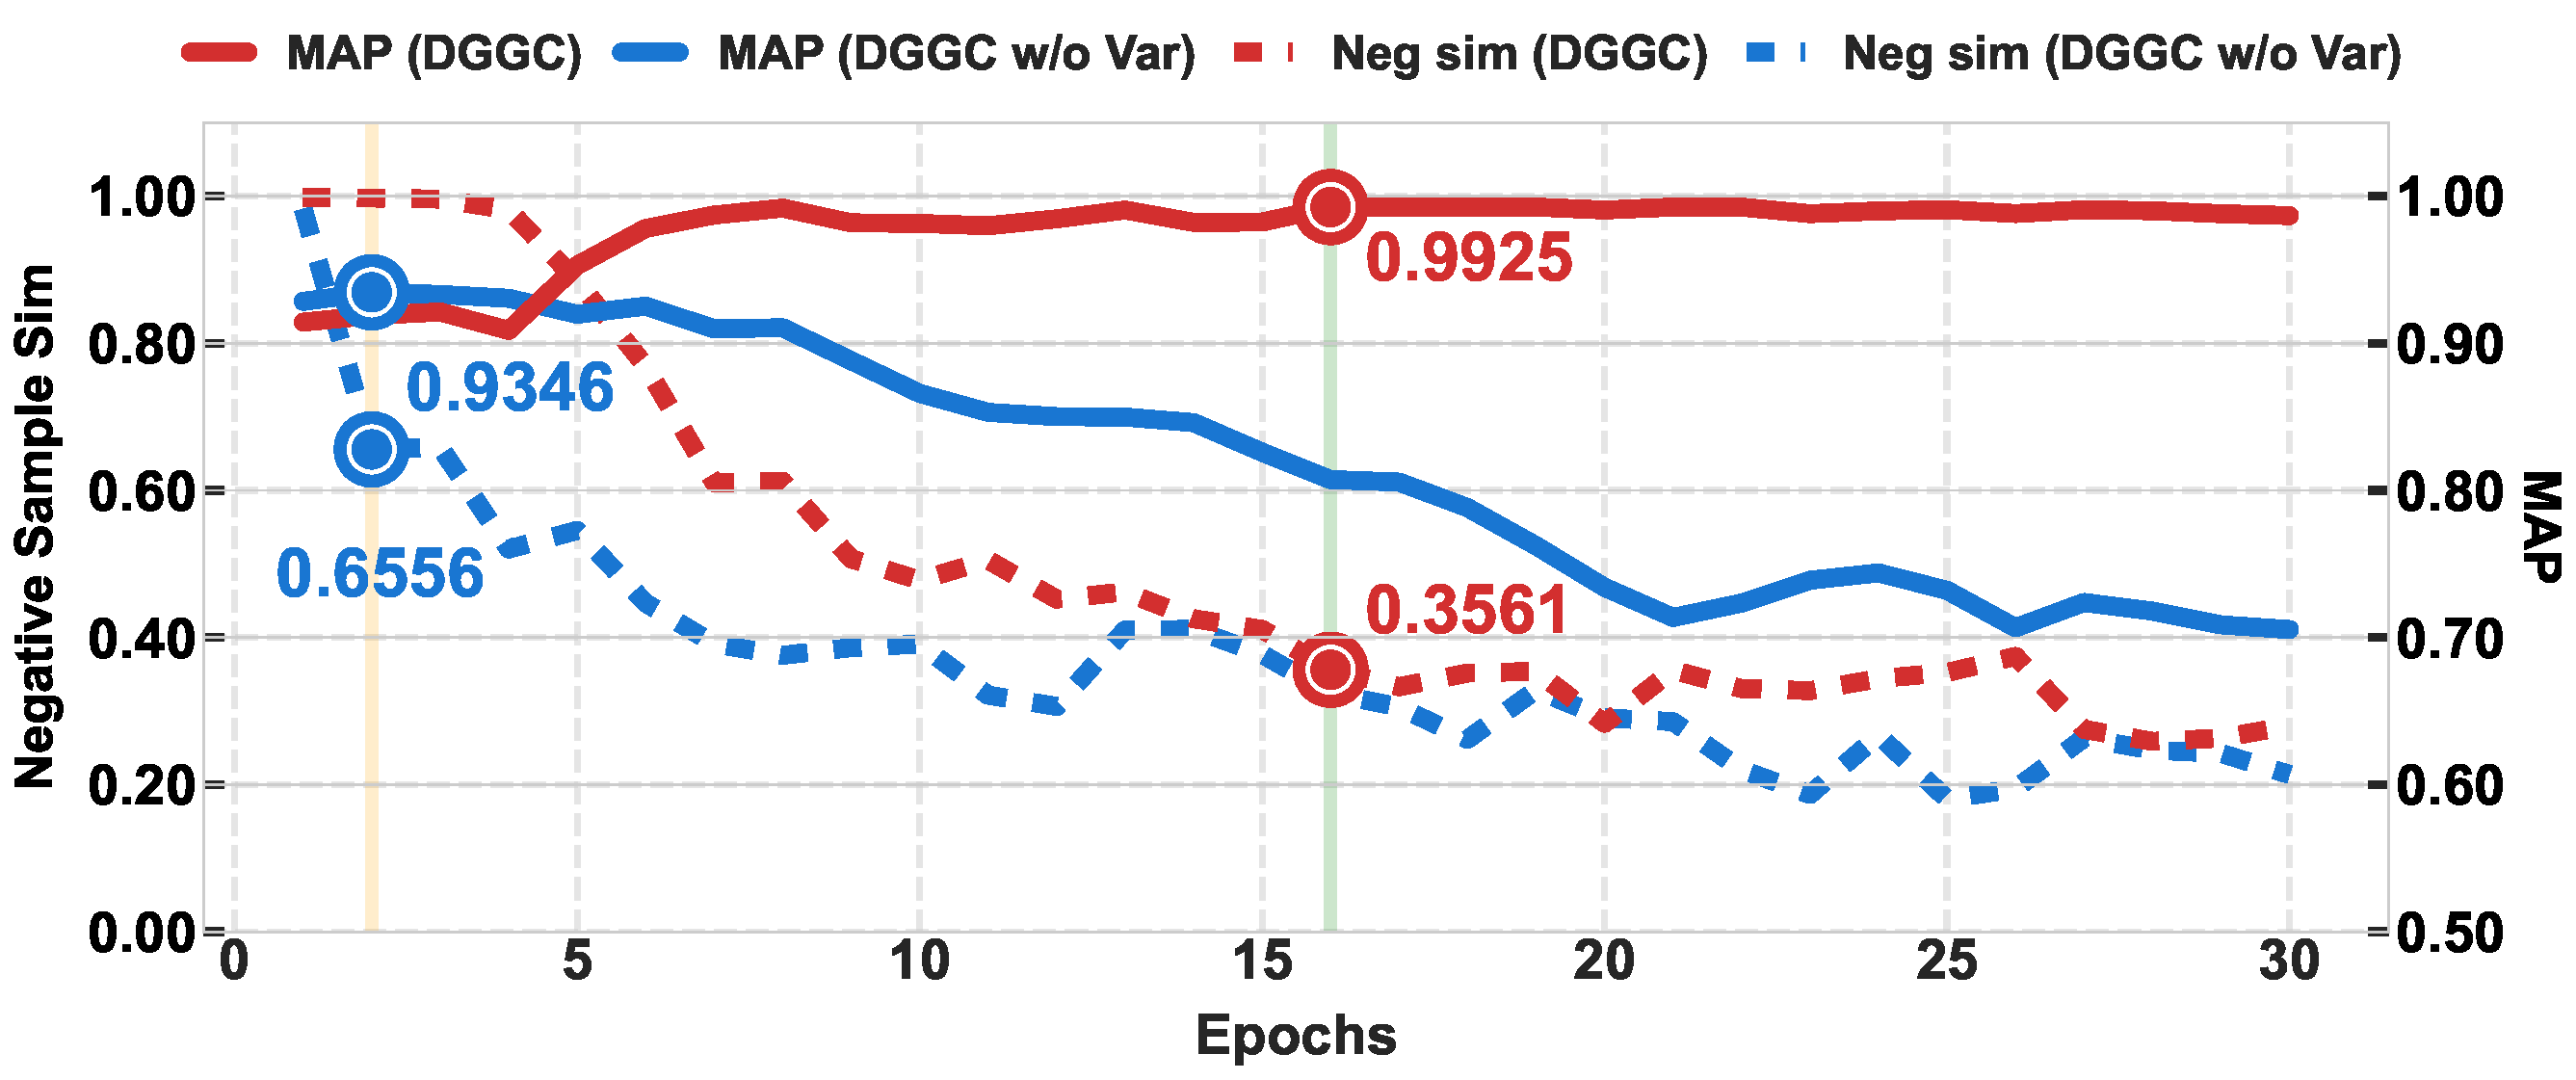
\includegraphics[width=.75\linewidth]{figure/case_study_epoch.pdf}
    \caption{The trend of cosine similarity among negative samples and the total MAP with the change of training epoch for the DGGC w/o Var and DGGC model. The light orange and light green vertical lines denote the epochs where the respective models achieve their optimal MAP performance. }
    \label{fig:case_study_epoch}
\end{figure}

In contrast, the DGGC model, which incorporates variance embeddings to account for semantic specificity, effectively captures the inconsistencies in table semantics illustrated in Figure \ref{fig:casestudy} (a) and (b). While both tables pertain to market entities, the query table emphasizes public wholesale markets, whereas Figure \ref{fig:casestudy} (b) focuses on more general contexts. The variance embedding in the loss function sensitively detects this mismatch. During training, the penalty term ($\lambda |\sigma_q - \sigma_n|_2$) in loss function actively separates the semantic centers, resulting in a significant reduction in cosine similarity from 0.9977 to 0.3561 (a 64.3\% decrease) between the tables while maintaining robust global performance, with MAP@k peaking at 0.9925. This successful filtering validates that introducing the variance constraint enables the model to distinguish between genuine semantic alignment \cite{karpukhin2020dense} and superficial lexical similarity \cite{robertson2009probabilistic}, which is critical for effective retrieval in real-world data lakes.

\fi

